\graphicspath{{003L/input/}}

%Custom prefix for tables and figures
\newcommand{\hbAppendixPrefix}{003L---D}



\renewcommand{\thefigure}{\hbAppendixPrefix\arabic{figure}}
\setcounter{figure}{0}
\renewcommand{\thetable}{\hbAppendixPrefix\arabic{table}} 
\setcounter{table}{0}

%Figure 3
\begin{figure}[H]
	\centering
	\includegraphics[width=0.8\textwidth]{Fig1}
	\caption{Long-term study site 003L near Cathedral Wash.  (A), Map showing surveyed area.  Shown are locations of monumented control points, remote camera, and the computational boundary (blue dashed line).  Aerial imagery collected in May 2013 at a steady discharge of 227 m3/s.  (B) 1 meter DEM derived from the March 28, 2008, survey of combined ground and bathymetric point data.  Shown on the sandbar are the water-surface elevations reached by discharges of 227 and 708 m3/s (red and yellow lines, respectively).  Water-surface elevations are derived from relations provided in Appendix C.  Survey dates and geomorphic attributes are provided in Appendix A.  Flow is right to left in both A and B.  River mile is in GCMRC convention, with river mile 0 at Lees Ferry, Arizona.}
\end{figure}


% Figure 2
\begin{figure}[H]
	\centering
	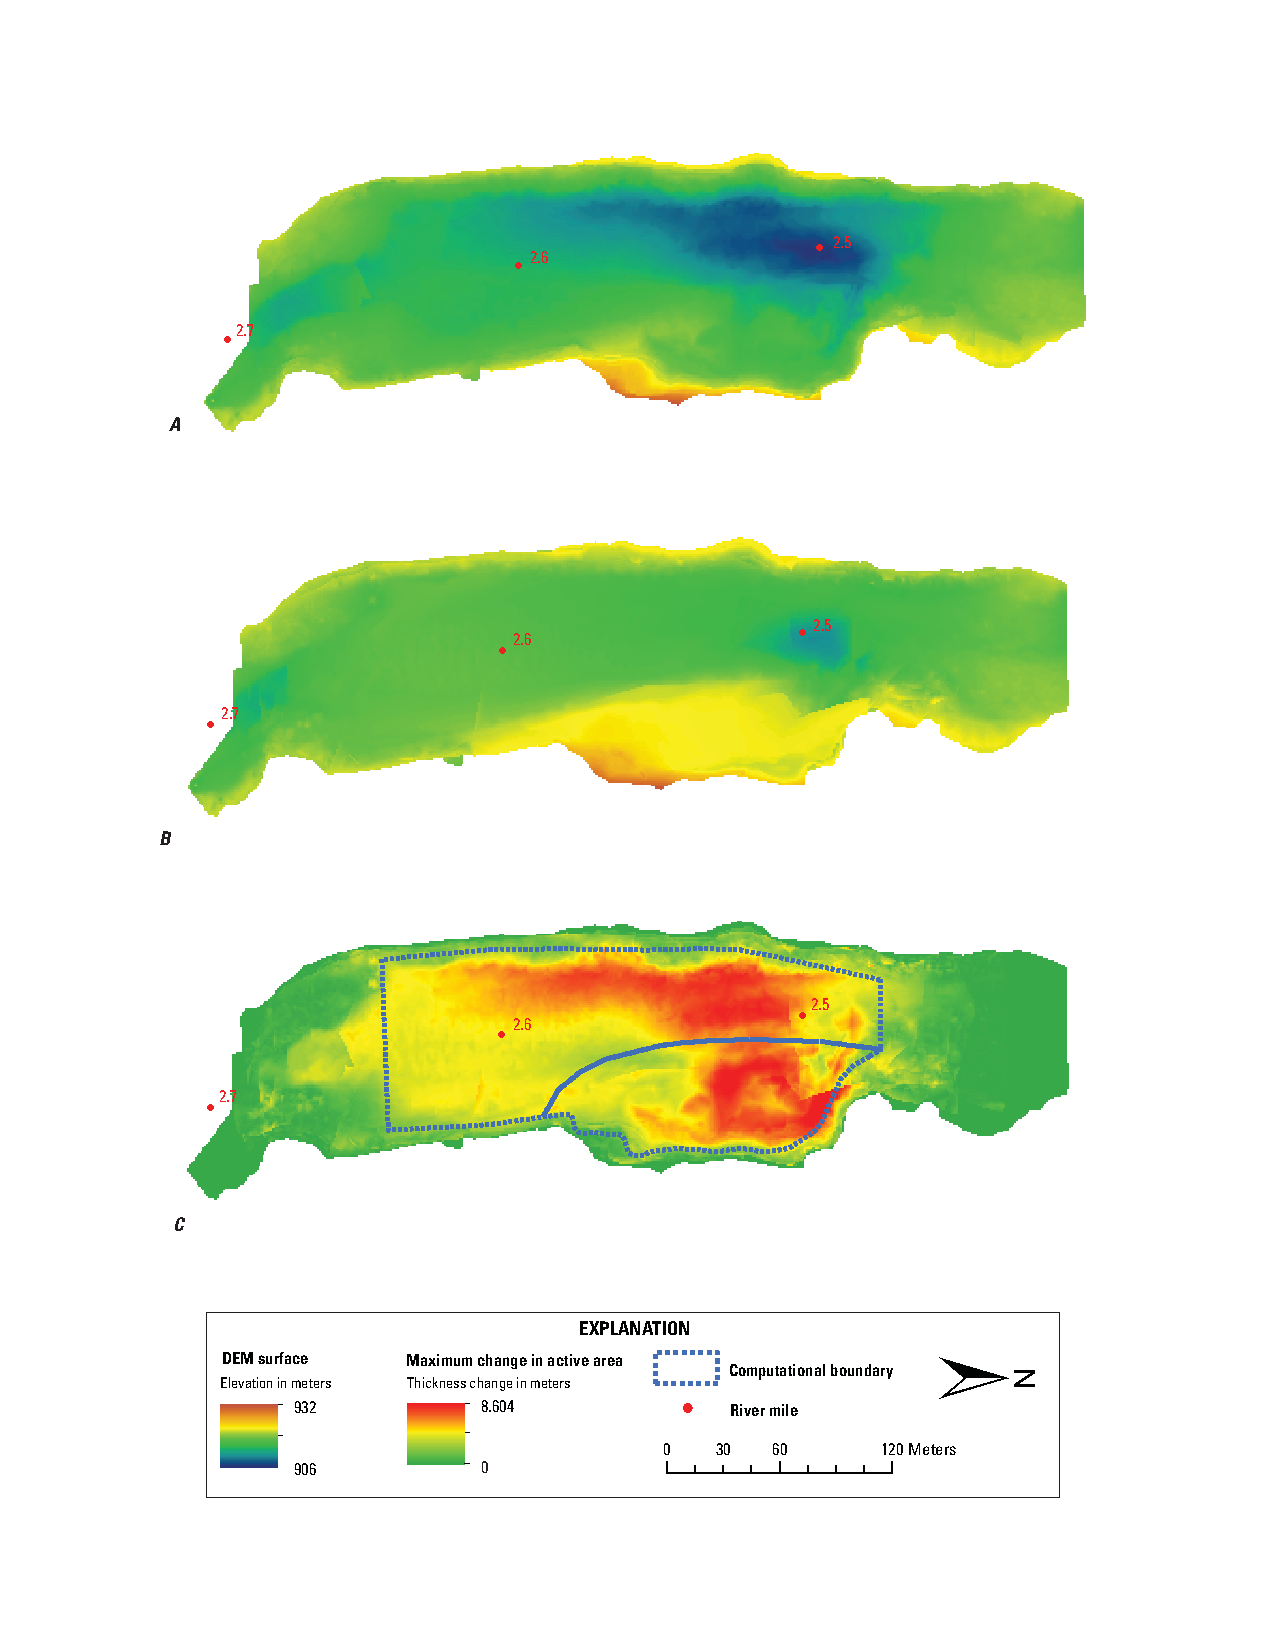
\includegraphics[width=0.8\textwidth]{Fig2}
	\caption{Long-term study site 003L near Cathedral Wash. Synthetic topography of the surveyed area in Fig. 003-D1 made by integrating the lowest and highest measured elevations collected since 1990 at 1-meter spaced grid nodes. (A) 1meter minimum surface DEM. (B) 1 meter maximum surface DEM. (C) Maximum potential active change based on subtracting the minimum (base level) surface from the maximum (potential) surface. The difference between these two surfaces is a conservative estimate of the maximum potential scour and fill, and thus of the active storage potential. The computational boundary is represented by the dashed blue line in C. Flow is right to left. River mile is in GCMRC convention, with river mile 0 at Lees Ferry, Arizona.}
\end{figure}


	%Figure 3
\begin{figure}[t!]
\centering
\subfigure[September 14, 1990]{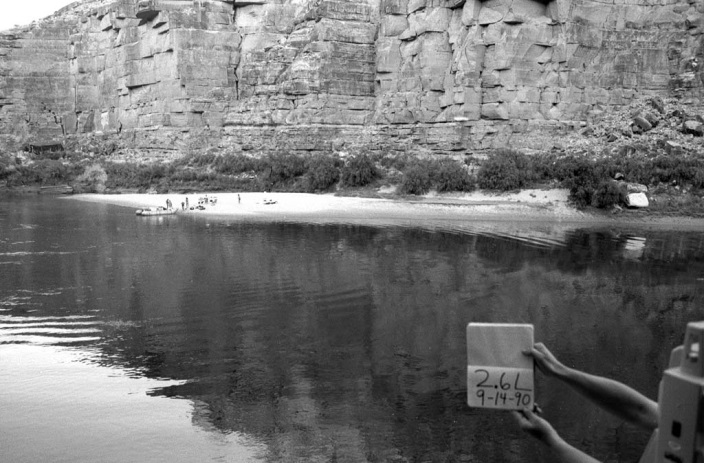
\includegraphics[width=3.2in]{image001}}
\subfigure[May 14, 1995]{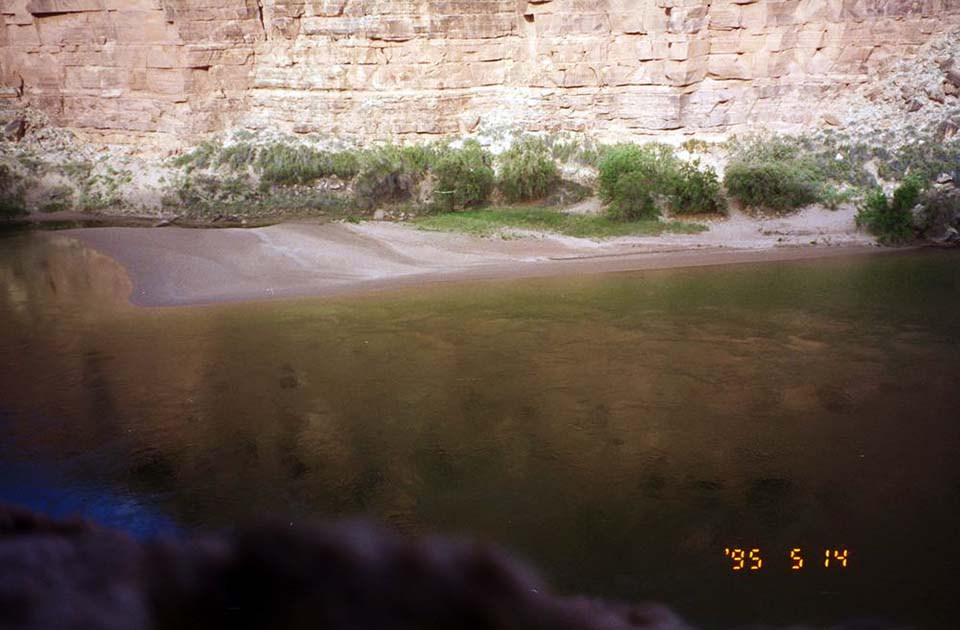
\includegraphics[width=3.2in]{image004}}
\subfigure[July 14, 1999]{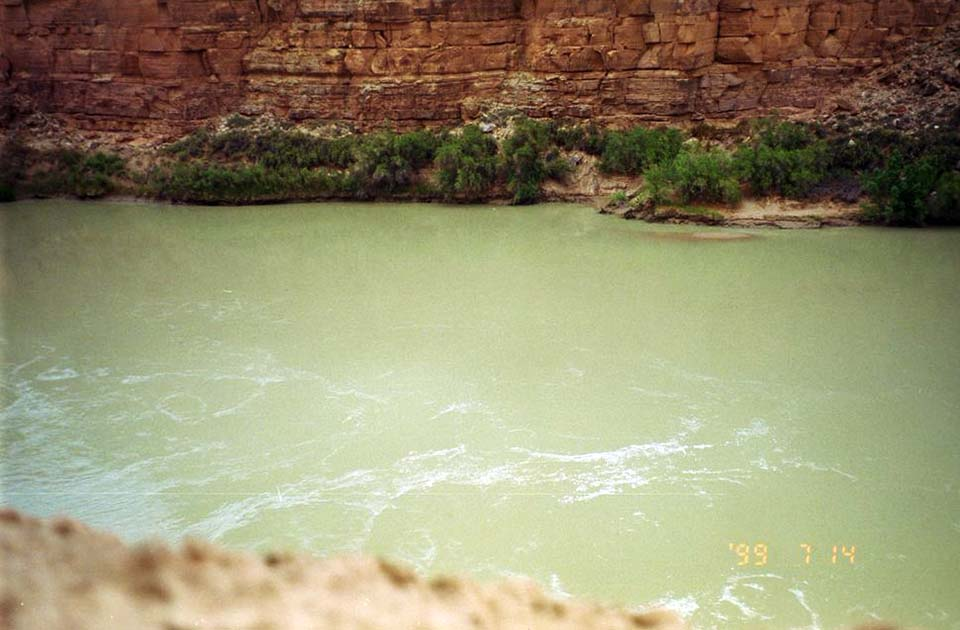
\includegraphics[width=3.2in]{image002}}
\subfigure[January 16, 2005]{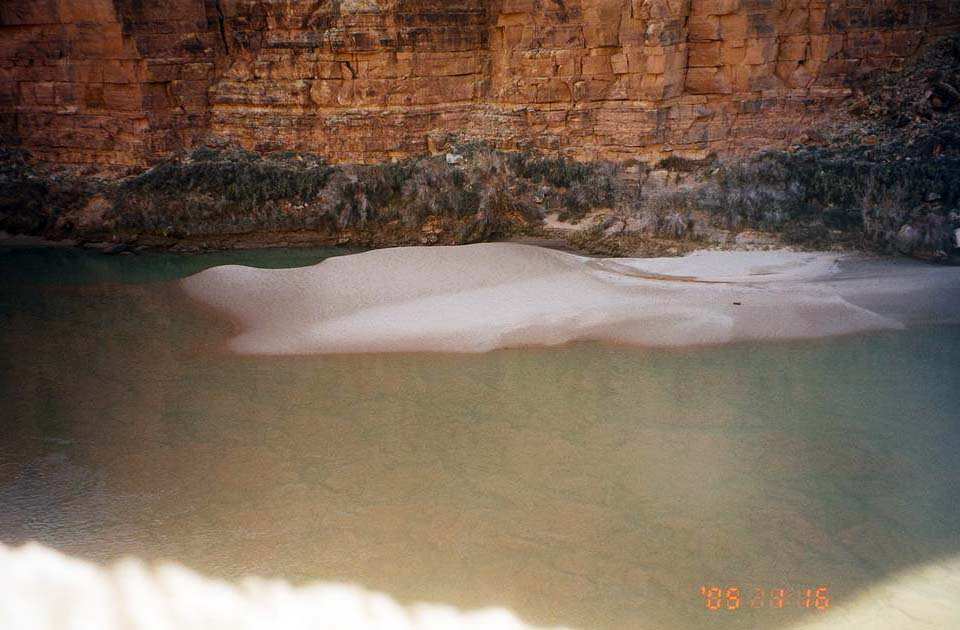
\includegraphics[width=3.2in]{image005}}
\subfigure[October 9, 2010]{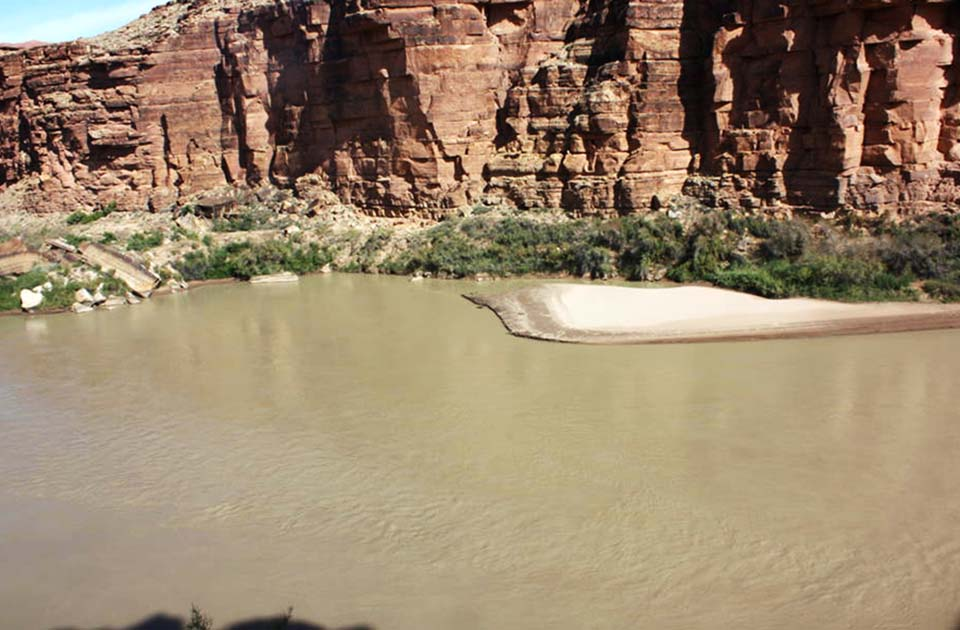
\includegraphics[width=3.2in]{image003}}
\subfigure[October 10, 2014]{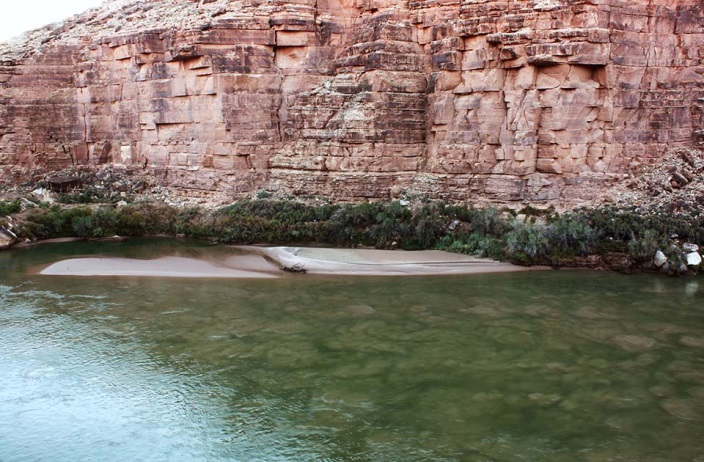
\includegraphics[width=3.2in]{image006}}
\caption{Selected photographs of long-term study site 003L near Cathedral Wash.  View is from the right bank of the river and shows the reattachment bar at various times between 1990 and 2014. Streamflow is from left to right.   }
\end{figure}
%Table1

\pgfkeysifdefined{/pgfplots/table/output empty row/.@cmd}{
	% upcoming releases offer this more convenient option:
	\pgfplotstableset{
		empty header/.style={
			every head row/.style={output empty row},
		}
	}
}


\clearpage

%%Table 1		
%\pgfplotstabletypeset[
%empty header,
%begin table=\begin{longtable},
%every first row/.append style={					
%				before row={
%						% First Page Header
%						\caption[Summary of Data Collected.]{Summary of Data collected. \newline Date of study is that of topographic survey (month-day-year).  Discharge at the time of each survey was estimated from the surveyed water surface elevation measured during topographic surveys and using the stage-discharge relations of Hazel and others (2006a).  Formative discharges were calculated by averaging the daily mean discharge at the nearest streamflow gaging station for the 30 days prior to the survey.  Peak discharge is the greatest recorded flow in between surveys.  {\checkmark} indicates data were collected. (-), indicates no data were collected or that data was not recoverable.} \\
%						\toprule
%							& Formative	&Peak		&Water Surface	& 			&\multicolumn{2}{c}{Bathymetric}	&				\\
%						Date&  Discharge&Discharge	&Elevation		& Discharge	&\multicolumn{2}{c}{Survey}		&Photographic	\\
%						\cmidrule(r){6-7}	
%							&  (m{$^3$})&(m{$^3$})	& (m)			&(m{$^3$})	&	SBES   &     MBES 							&Record			\\
%						\midrule\endfirsthead
%						
%						%All other page headers
%					    \multicolumn{8}{l}%
%					    {{Table \thetable\ Continued from previous page}} \\
%						\toprule
%						& Formative	&Peak		&Water Surface	& 			&\multicolumn{2}{c}{Bathymetric}	&				\\
%						Date&  Discharge&Discharge	&Elevation		& Discharge	&\multicolumn{2}{c}{Survey}		&Photographic	\\
%						\cmidrule(r){6-7}	
%						&  (m{$^3$})&(m{$^3$})	& (m)			&(m{$^3$})	&	SBES   &     MBES 							&Record			\\ 
%						\midrule\endhead
%						}
%						},
%columns/0/.style={string type},
%columns/1/.style={string type},
%columns/2/.style={string type},
%columns/3/.style={string type},
%columns/4/.style={string type},
%columns/5/.style={string type},
%columns/6/.style={string type},
%columns/7/.style={string type},
%every last row/.style={after row=\bottomrule},
%end table=\end{longtable},
%col sep=&, 
%]
%{
%	9-28-1990&372&835&920.351&140&&&
%	7-26-1991&428&575&920.339&137&&&
%	11-23-1991&268&527&921.090&278&&&
%	10-15-1992&287&459&921.531&368&&&{\checkmark}
%	4-1-1993&275&855&921.209&302&&&{\checkmark}
%	11-17-1993&281&470&921.437&348&{\checkmark}&&{\checkmark}
%	4-7-1994&283&419&921.214&303&{\checkmark}&&{\checkmark}
%	10-21-1994&260&450&920.838&229&{\checkmark}&&{\checkmark}
%	4-24-1995&294&498&920.895&240&{\checkmark}&&{\checkmark}
%	6-23-1995&414&507&922.269&534&{\checkmark}&&{\checkmark}
%	2-13-1996&426&580&921.574&377&{\checkmark}&&{\checkmark}
%	4-16-1996&613&1300&922.376&560&{\checkmark}&&{\checkmark}
%	9-13-1996&403&558&922.042&480&{\checkmark}&&{\checkmark}
%	2-14-1997&526&578&922.540&602&{\checkmark}&&{\checkmark}
%	4-20-1997&649&793&921.247&309&{\checkmark}&&{\checkmark}
%	8-24-1997&601&787&922.595&616&{\checkmark}&&{\checkmark}
%	11-3-1997&549&756&922.523&597&{\checkmark}&&{\checkmark}
%	11-6-1997&575&892&922.409&568&{\checkmark}&&{\checkmark}
%	4-15-1998&474&722&922.132&501&{\checkmark}&&{\checkmark}
%	5-6-1999&344&646&921.833&433&{\checkmark}&&{\checkmark}
%	3-18-2000&321&716&921.513&364&{\checkmark}&&{\checkmark}
%	6-2-2000&525&903&920.943&249&{\checkmark}&&{\checkmark}
%	8-19-2000&238&258&920.932&247&{\checkmark}&&{\checkmark}
%	9-9-2000&319&915&920.935&248&&{\checkmark}&{\checkmark}
%	10-5-2001&227&699&921.225&305&&&{\checkmark}
%	4-27-2002&291&408&921.339&328&&&{\checkmark}
%	9-20-2002&303&456&921.112&282&&{\checkmark}&{\checkmark}
%	4-25-2003&304&408&921.266&313&&&{\checkmark}
%	9-20-2003&303&479&920.994&259&&&{\checkmark}
%	6-1-2004&277&430&920.942&249&&&{\checkmark}
%	11-13-2004&228&487&921.113&283&&&{\checkmark}
%	12-2-2004&349&1195&921.410&342&&{\checkmark}&{\checkmark}
%	5-7-2005&238&578&921.404&341&&&{\checkmark}
%	10-7-2006&270&484&921.120&284&&&{\checkmark}
%	10-13-2007&290&470&920.936&248&&&{\checkmark}
%	2-2-2008&373&479&921.185&297&&{\checkmark}&{\checkmark}
%	3-28-2008&399&1254&921.187&297&&{\checkmark}&{\checkmark}
%	5-17-2008&367&399&921.163&293&&&{\checkmark}
%	10-11-2008&351&470&921.500&361&&&{\checkmark}
%	10-10-2009&291&419&921.155&291&&&{\checkmark}
%	10-5-2011&455&745&921.957&461&&&{\checkmark}
%	10-3-2012&227&603&920.848&231&&&{\checkmark}
%	9-21-2013&317&1277&921.475&356&&&{\checkmark}
%	9-24-2014&313&1065&921.715&407&&&{\checkmark}
%	9-23-2015&403&1082&921.814&429&&&{\checkmark}
%	}
%
%
%\pgfkeysifdefined{/pgfplots/table/output empty row/.@cmd}{
%	% upcoming releases offer this more convenient option:
%	\pgfplotstableset{
%		empty header/.style={
%			every head row/.style={output empty row},
%		}
%	}
%}

\input{003L/input/table1}
 \clearpage
 



\input{003L/input/table2}

